In this calculator, loss exceedance curves and loss maps for various return periods can be calculated, based on probabilistic seismic hazard, with an event-based approach. A large number of stochastic event sets are generated, and the associated ground motion fields for each event are used together with a vulnerability model to compute the individual (per asset) and total (sum of all the losses per event) losses. Then, this distribution of losses is employed to derive a loss exceedance curve per asset, as well as a total loss exceedance curve representative of the complete building portfolio. Furthermore, oq-risklib can also compute loss maps for various return periods by interpolating each individual loss curve with the respective probability of exceedance. In Figure~\ref{fig:ProbEvent}, the input/output scheme of this calculator is illustrated.

\begin{figure}[ht]
\centering
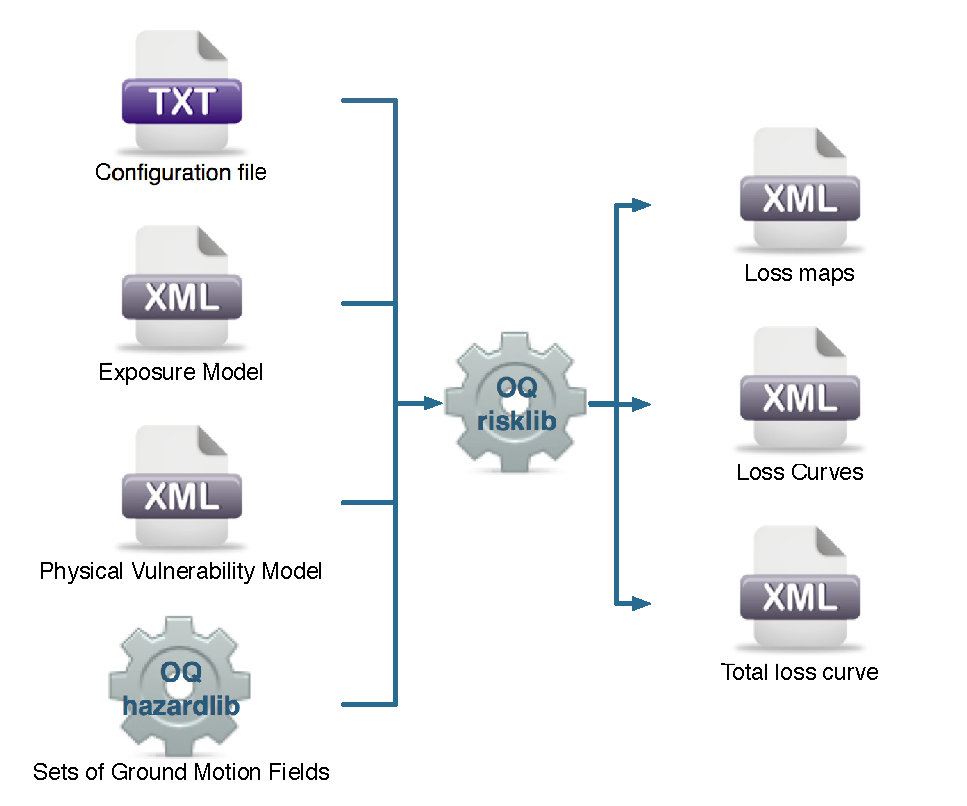
\includegraphics[width=9cm,height=7cm]{figures/risk/ProbEvent.pdf}
\caption{Probabilistic Event-based Risk Calculator input/output structure.}
\label{fig:ProbEvent}
\end{figure}